\begin{question}[section=11,name={Antennengewinn 2},difficulty=,quantity=2,type=thr,tags={20130625}]
	Geben Sie zwei praxisgerechte Verfahren für die Bestimmung des Antennengewinnes an (Skizze). Welche Länge muss das für die Messung verwendete Funkfeld haben?
	\\ \textbf{Hinweis:}\\
	Skript Seite 107
\end{question}
\begin{solution}
	\begin{figure}[H]
		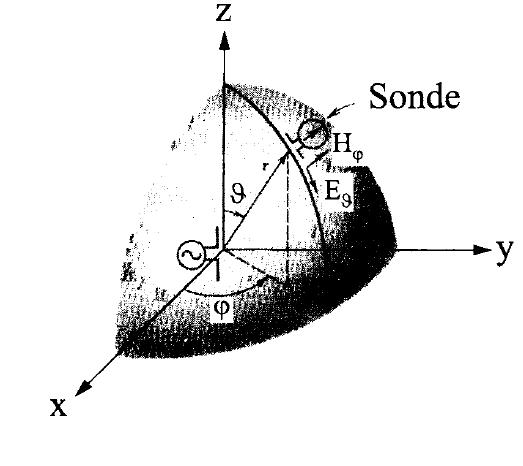
\includegraphics[width=14cm]{./opn/exm/thr/chp/11/2/bild.jpeg}
	\end{figure}
	Da es sich um das Fernfeld handelt, muss die Distanz größer als die Raylighdistanz sein.\\
	\begin{itemize}
		\item{Feldstärke (im Fernfeld) zur Feldstärke der Vergleichsantenne bei gleicher Leistung am Eingang.}
		\item{Einsparung an verfügbarer Leistung für die Versuchsantenne gegenüber Vergleichsantenne bei gleicher Fernfeldstärke}
	\end{itemize}
\end{solution}